\begin{slide}[toc=PRNG]{Pseudorandom number generator}
\null\vfill

  \begin{itemize}
    \item PRNG is an algorithm for generating a sequence of ``random'' numbers
    \item Example: middle-square method (used in ENIAC)
    \begin{itemize}
      \item take $n$-digit number as your seed
      \item square it to get $2n$-digit number (add leading zeroes if necessary)
      \item $n$ middle digits are the result and the seed for next number
    \end{itemize}
    \item Middle-square method for $n = 4$ and base seed = $1111$:
  \end{itemize}
  \vspace{-10pt}
  \begin{eqnarray*}
    1111^2 & = & {\color{pdcolor3}01}2343{\color{pdcolor3}21} \rightarrow 2343 \\
    2343^2 & = & {\color{pdcolor3}05}4896{\color{pdcolor3}49} \rightarrow 4896 \\
    & \vdots & \\
    1111^2 & = & {\color{pdcolor3}01}2343{\color{pdcolor3}21} \rightarrow 2343 
  \end{eqnarray*}
    
\vfill\null
\end{slide}

\begin{slide}[toc=]{Pseudorandom number generator}
\null\vfill

  \begin{itemize}
    \item Nowadays, more sophisticated PRNGs exist, but they also suffer on some common problems:
    \begin{itemize}
      \item periodicity / different periodicity for different base seed
      \item nonuniformity of number distributions
      \item correlation of successive numbers
    \end{itemize}
  \end{itemize}

  \twocolumn
  {
    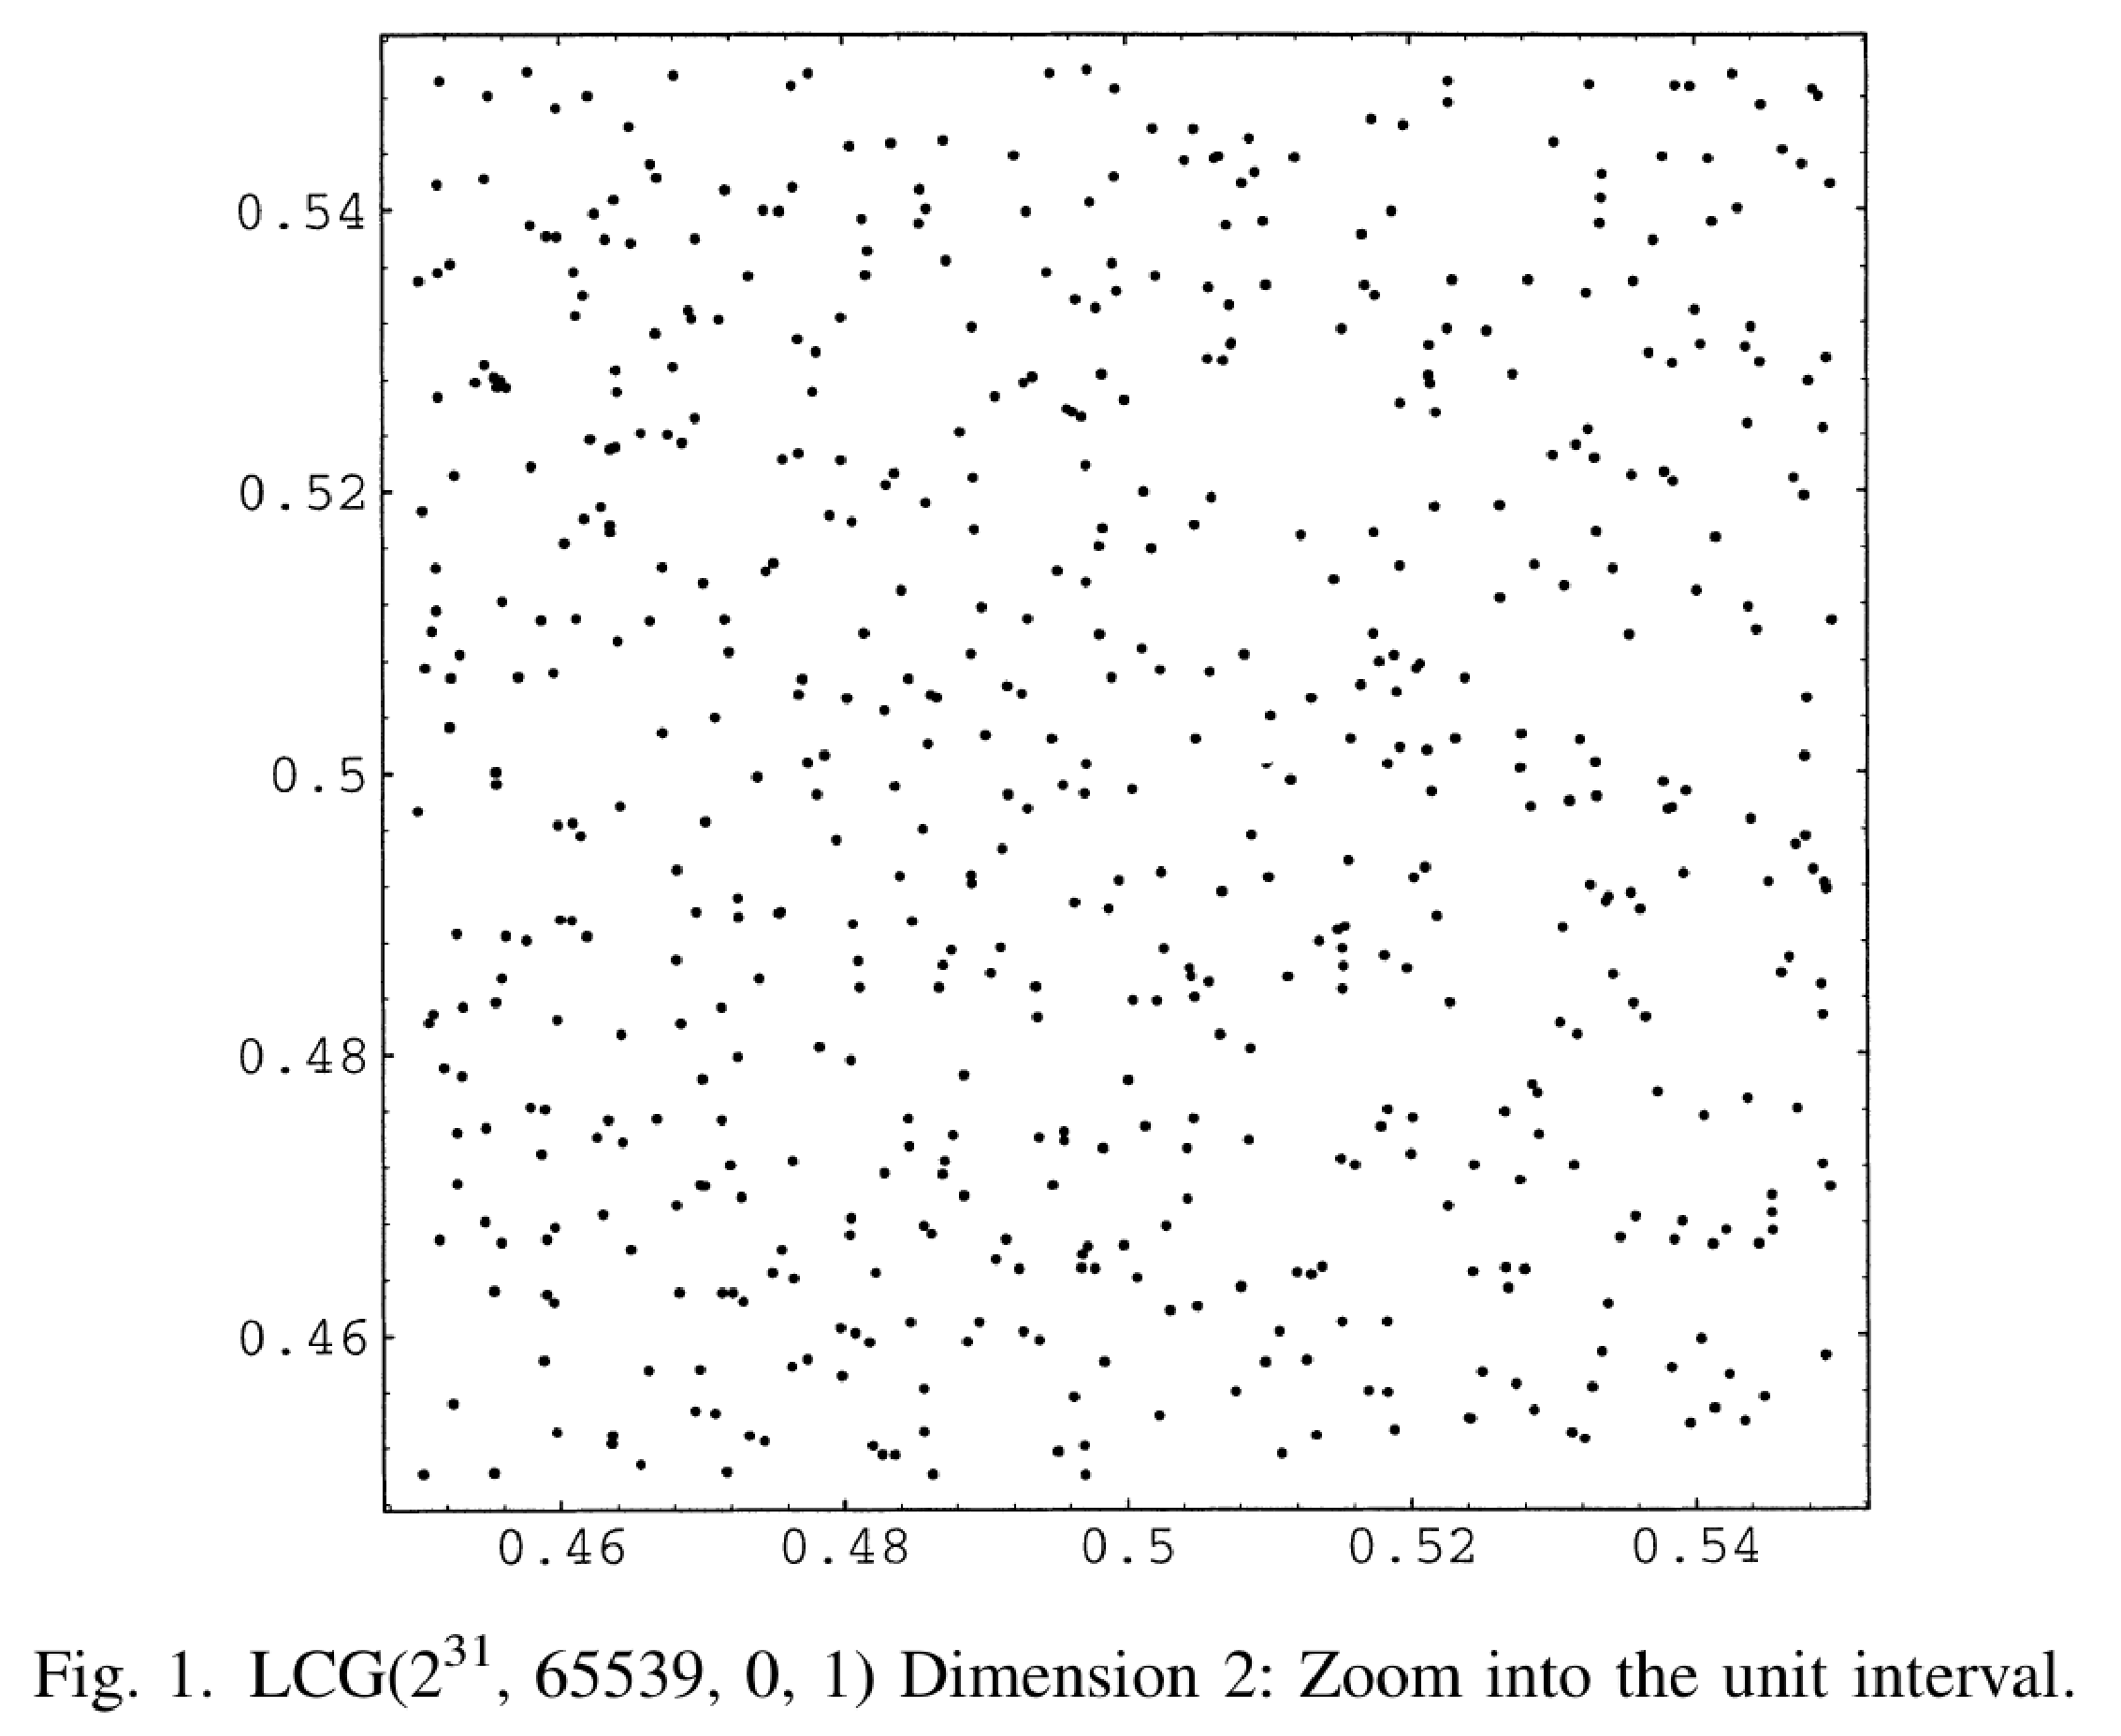
\includegraphics[width=\columnwidth]{figures/random2d.eps}
  }
  {
    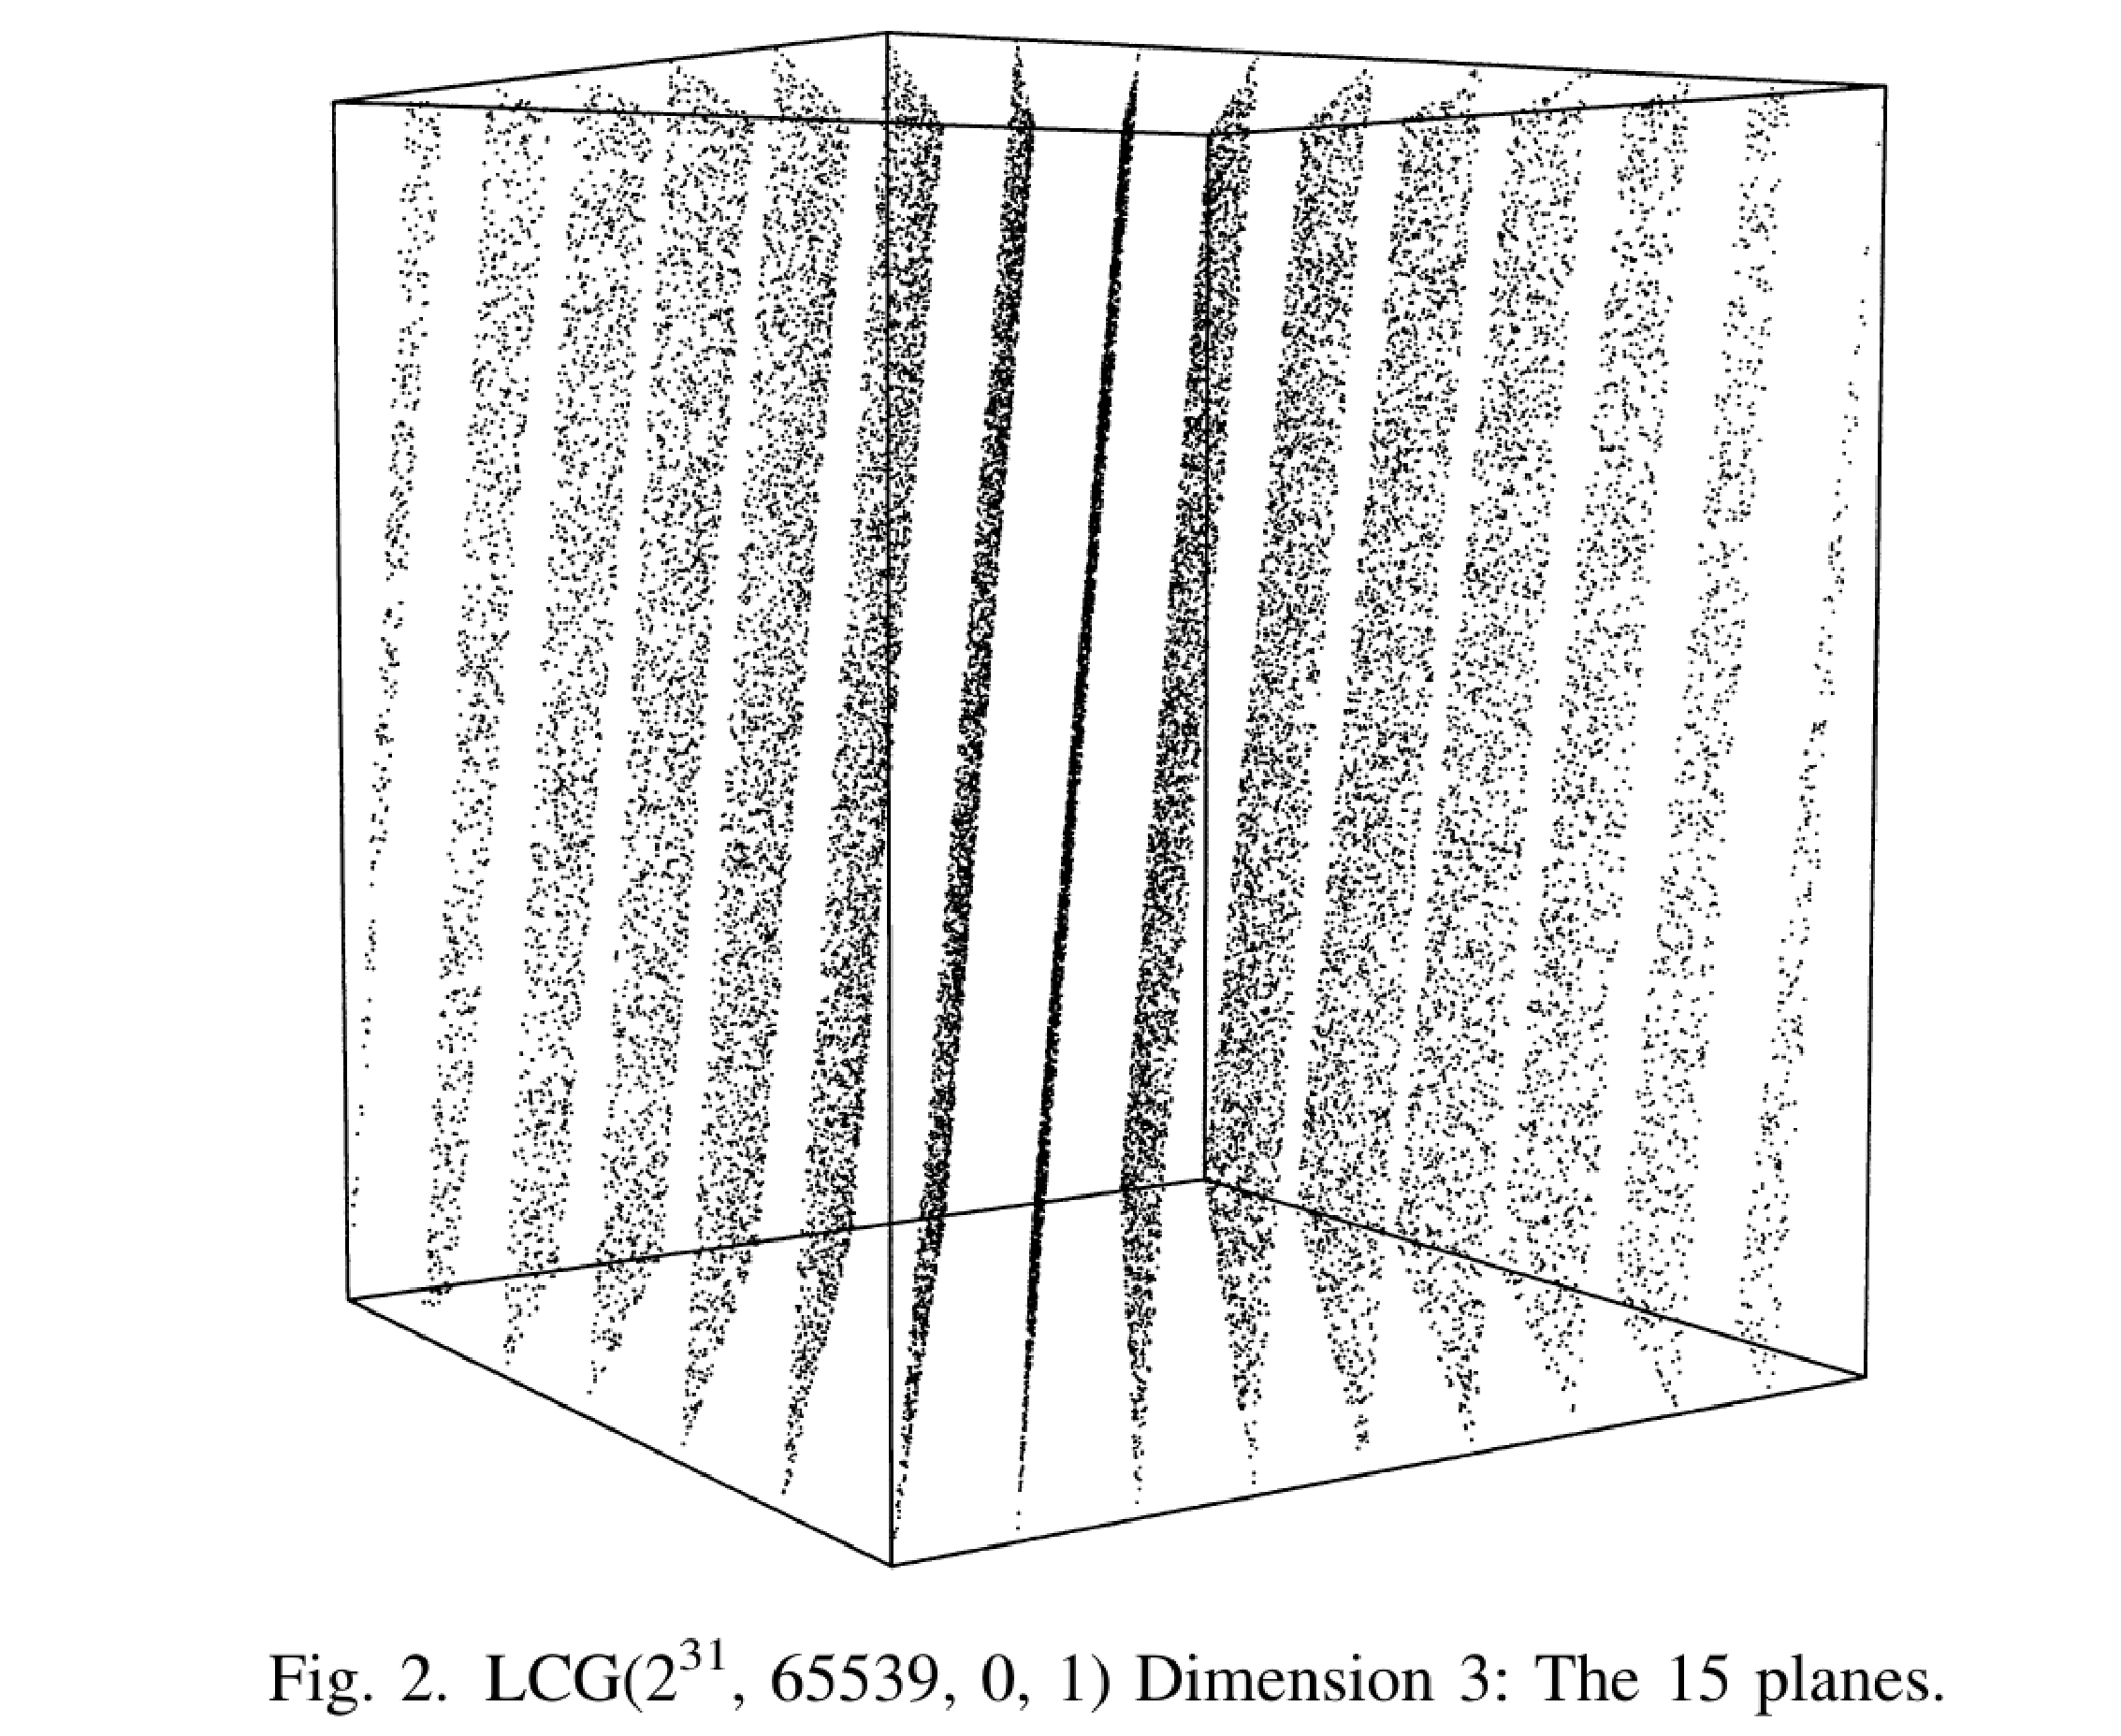
\includegraphics[width=\columnwidth]{figures/random3d.eps}
  }
  {\it\color{pdcolor3}Mathematics and Computers in Simulations 46 (1998) 485-505}
\vfill\null
\end{slide}
